\documentclass[12pt, notitlepage, final]{article} 

\newcommand{\name}{Vince Coghlan}

\usepackage{amsfonts}
\usepackage{amssymb}
\usepackage{amsmath}
\usepackage{latexsym}
\usepackage{enumerate}
\usepackage{amsthm}
\usepackage{nccmath}
\usepackage{setspace}
\usepackage[pdftex]{graphicx}
\usepackage{epstopdf}
\usepackage[siunitx]{circuitikz}
\usepackage{tikz}
\usepackage{float}
\usepackage{cancel}
\usepackage{pgfplots}
\usepackage{setspace}
\usepackage{overpic}
\usepackage{mathtools}
\usepackage{listings}
\usepackage{color}

\numberwithin{equation}{section}
\DeclareRobustCommand{\beginProtected}[1]{\begin{#1}}
\DeclareRobustCommand{\endProtected}[1]{\end{#1}}
\newcommand{\dbr}[1]{d_{\mbox{#1BR}}}
\newtheorem{lemma}{Lemma}
\newtheorem*{corollary}{Corollary}
\newtheorem{theorem}{Theorem}
\newtheorem{proposition}{Proposition}
\theoremstyle{definition}
\newtheorem{define}{Definition}
\newcommand{\column}[2]{
\left( \begin{array}{ccc}
#1 \\
#2
\end{array} \right)}

\newdimen\digitwidth
\settowidth\digitwidth{0}
\def~{\hspace{\digitwidth}}

\setlength{\parskip}{1pc}
\setlength{\parindent}{0pt}
\setlength{\topmargin}{-3pc}
\setlength{\textheight}{9.0in}
\setlength{\oddsidemargin}{0pc}
\setlength{\evensidemargin}{0pc}
\setlength{\textwidth}{6.5in}
\newcommand{\answer}[1]{\newpage\noindent\framebox{\vbox{{\bf ECEN 4797 Fall 2014}
\hfill {\bf \name} \vspace{-1cm}
\begin{center}{Homework \#2}\end{center} } }\bigskip }

%absolute value code
\DeclarePairedDelimiter\abs{\lvert}{\rvert}%
\DeclarePairedDelimiter\norm{\lVert}{\rVert}
\makeatletter
\let\oldabs\abs
\def\abs{\@ifstar{\oldabs}{\oldabs*}}
%
\let\oldnorm\norm
\def\norm{\@ifstar{\oldnorm}{\oldnorm*}}
\makeatother

\def\dbar{{\mathchar'26\mkern-12mu d}}
\def \Frac{\displaystyle\frac}
\def \Sum{\displaystyle\sum}
\def \Int{\displaystyle\int}
\def \Prod{\displaystyle\prod}
\def \P[x]{\Frac{\partial}{\partial x}}
\def \D[x]{\Frac{d}{dx}}
\newcommand{\PD}[2]{\frac{\partial#1}{\partial#2}}
\newcommand{\PF}[1]{\frac{\partial}{\partial#1}}
\newcommand{\DD}[2]{\frac{d#1}{d#2}}
\newcommand{\DF}[1]{\frac{d}{d#1}}
\newcommand{\fix}[2]{\left(#1\right)_#2}
\newcommand{\ket}[1]{|#1\rangle}
\newcommand{\bra}[1]{\langle#1|}
\newcommand{\braket}[2]{\langle #1 | #2 \rangle}
\newcommand{\bopk}[3]{\langle #1 | #2 | #3 \rangle}
\newcommand{\Choose}[2]{\displaystyle {#1 \choose #2}}
\newcommand{\proj}[1]{\ket{#1}\bra{#1}}
\def\del{\vec{\nabla}}
\newcommand{\avg}[1]{\langle#1\rangle}
\newcommand{\piecewise}[4]{\left\{\beginProtected{array}{rl}#1&:#2\\#3&:#4\endProtected{array}\right.}
\newcommand{\systeme}[2]{\left\{\beginProtected{array}{rl}#1\\#2\endProtected{array}\right.}
\def \KE{K\!E}
\def\Godel{G$\ddot{\mbox{o}}$del}

\onehalfspacing

\begin{document}

\answer{}

\textbf{2.1:} In the converter of Fig 3.31, the inductor has winding resistance $R_L$.  All
other losses can be ignored.  The switches operate synchronously: each is in position 1 for
$0 < t < DT_g$, and in position 2 for $DT_g < t < T_g$.
\begin{center}
  \begin{circuitikz}[american]
 \draw
 (0,0) to [V,v=$V_g$] (0, 3) {}
   to [L=$L$] (3, 3) {}
   to [short] (8, 3) {}
   to [short, -*] (8, 2.25) {}
 (0,0) to [short] (8, 0) {}
   to [short, -*] (8, 0.75) {}
 (3, 3) to [short, -*] (3, 2.25) {}
 (3, 0) to [short, -*] (3, 0.75) {}
 (3.75, 1.5) to [short, *-] (4.25, 1.5) {}
   to [short] (4.25, 2) {}
   to [C=$C$] (6.75, 2) {}
   to [short] (6.75, 1) {}
   to [R=$R$] (4.25, 1) {}
   to [short] (4.25, 1.5) {}
 (6.75, 1.5) to [short, -*] (7.25, 1.5) {}
   to [short] (8.15, 2.2) {}
 (3.75, 1.5) to [short] (2.85, 0.85) {}
;\end{circuitikz}
\end{center}

\begin{enumerate}[(a)]
  \item{Derive an expression for the nonideal voltage conversion ratio $V/V_g$.}\\
  In one state of the converter:
  \begin{center}
    \begin{circuitikz}[american]
   \draw
   (0,0) to [V,v=$V_g$] (0, 3) {}
     to [L=$L$] (3, 3) {}
     to [short] (6, 3) {}
     to [R=$R$,v=$V$] (6, 0) {}
     to [short] (0, 0) {}
   (3, 3) to [C=$C$] (3, 0) {}
  ;\end{circuitikz}
  \end{center}
  in the otehr state:
  \begin{center}
    \begin{circuitikz}[american]
   \draw
   (0,0) to [V,v=$V_g$] (0, 3) {}
     to [L=$L$] (3, 3) {}
     to [short] (6, 3) {}
   (6, 0) to [R=$R$, v=$V$] (6, 3) {}
   (6, 0) to [short] (0, 0) {}
   (3, 3) to [C=$C$] (3, 0) {}
  ;\end{circuitikz}
  \end{center}
  Using KVL:
  \[
    V_L = V_g - i_LR_L-V\text{ and }V_L = V_g - i_LR_L + V
  \]
  \[
    D(V_g - i_LR_L - V) + (1-D)(V_g - i_LR_L+V) = 0
  \]
  \[
    DV_g - Di_LR_L - DV + V_g - i_LR_L + V - DV_g + Di_LR_L - DV = 0
  \]
  \[
    -2DV+V_g-i_LR_L+V=0
  \]
  Using KCL:
  \[
    i_C=i_L+\frac{V}{R}\text{ and }i_C=i_L-\frac{V}{R}
  \]
  \[
    D(i_L-\frac{V}{R}) + (1-D)(i_L+\frac{V}{R}) = 0
  \]
  \[
    \frac{-2DV}{R} + i_L + \frac{V}{R} = 0 \Rightarrow i_L = (2D-1)\frac{V}{R}
  \]
  Two equations, two unknowns, we can plug and go:
  \[
    -2DV+V_g-(2D-1)\frac{V}{R}R_L+V=0
  \]
  \[
    V_g = 2DV+(2D-1)\frac{VR_L}{R} - V
  \]
  \[
    \frac{V}{V_g} = \frac{1}{2D + (2D-1)\frac{R_L}{R} - 1} = \frac{1}{(2D-1)(1+\frac{R_L}{R})}
  \]

  \item{Plot your result of part (a) over the range $0 < D \leq 1$, for $R_L/R = 0.001$, amd 0.05.}\\
    For $\frac{R_L}{R} = 0.001$, we find:
    \begin{figure}[H]
    \begin{center}
    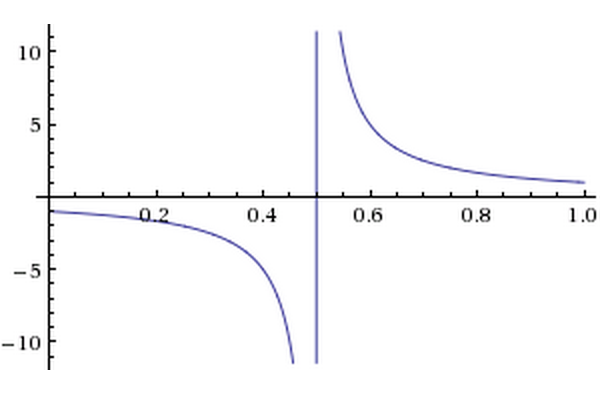
\includegraphics[width=8cm]{f1}
    \end{center}
    \end{figure}
    For 0.05, we find:
    \begin{figure}[H]
    \begin{center}
    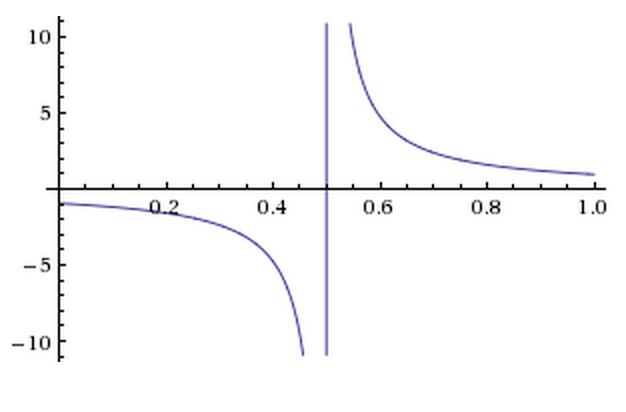
\includegraphics[width=8cm]{f2}
    \end{center}
    \end{figure}
  \item{Derive an expression for the efficiency. Manipulate your expression into a form similar
    to Eq. (3.35)}\\
    Luckily for us, the same current is always flowing through $L$.
    \[
      \eta = \frac{P_{in}}{P_{out}}
    \]
    \[
      P_{in} = V_g\cdot I_L
    \]
    \[
      P_{out} = V\cdot I_L
    \]
    \[
      \eta = \frac{V_g}{V} = (2D-1)(1+\frac{R_L}{R})
    \]
    It makes sense that at .5 duty cycle, no power would be transmitted, and the efficiency would be 0.
    \end{enumerate}

    \textbf{2.2:} The inductor in the converter of Fig. 3.31 has winding resistance $R_L$.  All other losses can
    be ignored.  Derive an equivalent circuit model for this converter.
    \begin{center}
     \begin{circuitikz}[american]
     \draw
     (4, 3) node[transformer](T) {} node[above] {$(2D - 1):1$}
     (0,0.9) to [V,v=$V_g$] (0, 3) {}
       to [R=$R_L$] (T.A1)
     (T.B1) to [short] (6, 3) {}
       to [R=$R$] (6, 0.9) {}
       to [short] (T.B2)
     (0,0.9) to [short] (T.A2)
         ;\end{circuitikz}
    \end{center}

    \textbf{2.3:} A 1.5V battery is used to power a 5V, 1A load.  It has been decided
    to use a buck-boost converter in this application.  A suitable transistor is found
    with an on-resistance of $35 m\Omega$, and a Schottky diode is found with a forward
    drop of 0.5V. The on-resistance of the Schottky diode may be ignored. The power
    stage schematic is shown in Fig. 3.34.

    \begin{enumerate}[(a)]
      \item{Derive an equivalent circuit that models the dc properties of this converter.
        Include the transistor and diode conduction losses, as well as the inductor copper
      loss, but ignore all other sources of loss. Your model should correctly describe the
      converter dc input port.}\\
      If we split up the circuit, we can do some analysis, using KVL:
      \[
        v_L = V_g - i_LR_L-i_LR_{on}\text{ and }v_L = V+V_D
      \]
      \[
        D(V_g - i_LR_L-i_LR_{on}) + D'(V+V_D) = 0
      \]
      using KCL:
      \[
        i_c = \frac{V}{R}\text{ and }i_c=\frac{V}{R}-i_L
      \]
      \[
        D(\frac{V}{R}) + D'(\frac{V}{R}-i_L) = 0
      \]

      \begin{center}
      \begin{circuitikz}[american]
       \draw
       (6, 3) node[transformer](T) {} node[above] {$D':1$}
       (0,0.9) to [V,v=$DV_g$] (0, 3) {}
         to [R=$DR_L$] (2, 3)
         to [R=$DR_{on}$] (4, 3)
         (T.A1) to [V=$D'V_{D}$] (4, 3)
       (T.B1) to [short] (8, 3) {}
         to [R=$R$] (8, 0.9) {}
         to [short] (T.B2)
       (0,0.9) to [short] (T.A2)
      ;\end{circuitikz}
    \end{center}
    \item{It is desired that the converter operate with at least 70\% efficiency
      under normal conditions (i.e., when the input voltage is 1.5 V and the output voltage
    is 5V at 1 A). How large can the inductor winding resistance be? At what duty cycle will
    the converter then operate? \emph{Note:} there is an easy way and a not-so-easy way to
    analytically solve this part.}\\
    We know that the output power is $P_{out} = IV = 5W$.  We can work backwards to account
    for power loss in every component in the circuit.
    \[
      \eta = \frac{P_{out}}{P_{in}} = 0.7 = \frac{5}{P_{in}} \Rightarrow P_{in} = \frac{5}{0.7}\Rightarrow I_{in} = \frac{5/.7}{1.5}
    \]
    \[
      \frac{5}{.7} = \frac{5/.7}{1.5}(0.035) + (\frac{5/.7}{1.5}-1)R_L + (1\cdot0.5) + 5
    \]
    \[
      R_L = 0.3924\Omega
    \]
    \end{enumerate}


\end{document}
